\section{Evaluation and benchmarking}

In order to develop a robust system, we have decided to focus on intensive testing and evaluation. 
Therefore, we tried to find possible ways to build a test arena and equip it with real objects.
However, this is impossible for us due to a strongly limited budget and lack of space. 
However, we came up with a better idea - we have decided to use one of our flats, see Fig.~\ref{fig:kitchen}.
%Hence, our robot is deployed permanently in this flat now and we record datasets during regular testing which we plan to publish later. 

We have found such an environment which is similar to the arena with all of the tricky situations such as narrow corridors, door steps, a large mirror, etc. 
Therefore, we are able to test our algorithms in a realistic environment and improve their robustness.
%A more detailed description of our evaluation will be published there before the competition in November.

\begin{figure}[!htb]
\centering
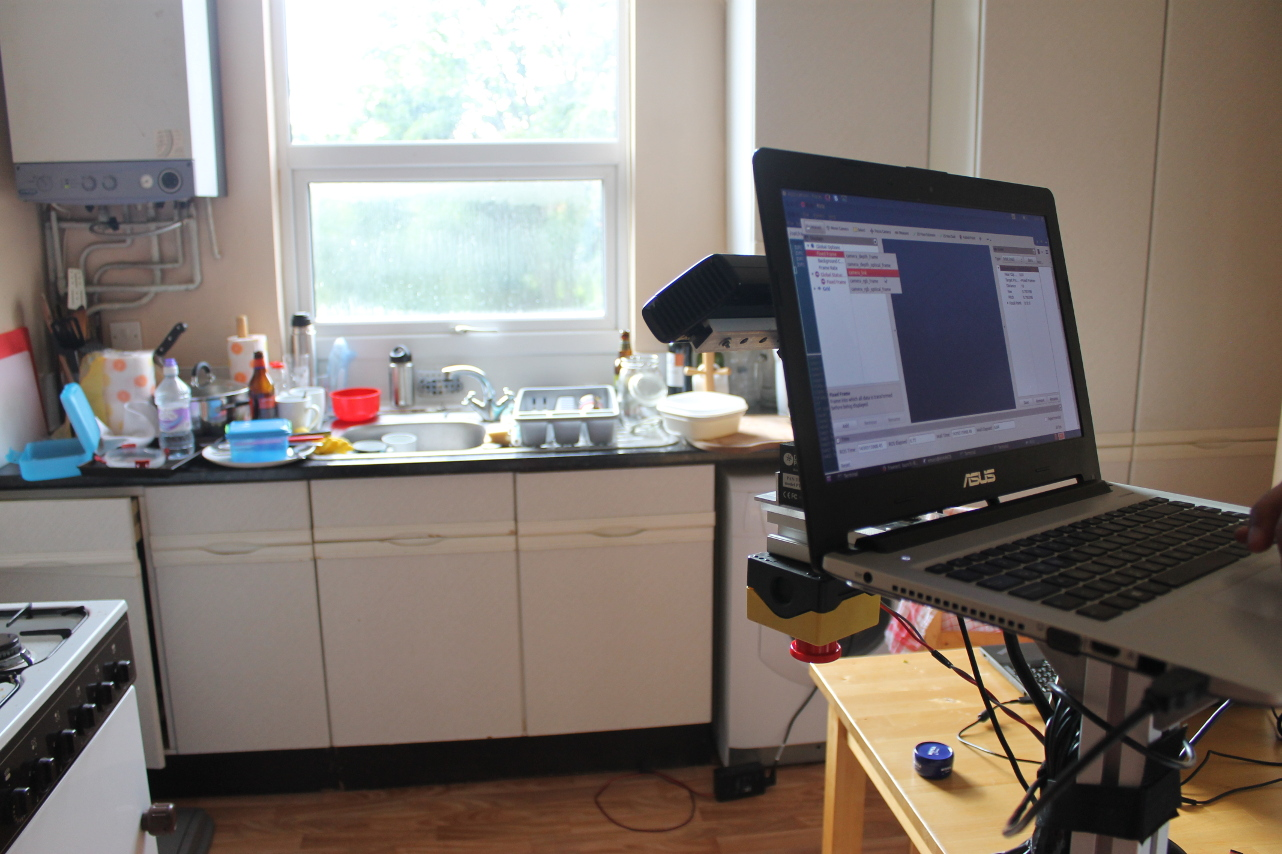
\includegraphics[width=3.in]{kitchen.JPG}
\caption{Long-term deployment of Dora in a flat}
\label{fig:kitchen}
\end{figure}  